% Options for packages loaded elsewhere
% Options for packages loaded elsewhere
\PassOptionsToPackage{unicode}{hyperref}
\PassOptionsToPackage{hyphens}{url}
\PassOptionsToPackage{dvipsnames,svgnames,x11names}{xcolor}
%
\documentclass[
  letterpaper,
  DIV=11,
  numbers=noendperiod]{scrreprt}
\usepackage{xcolor}
\usepackage{amsmath,amssymb}
\setcounter{secnumdepth}{5}
\usepackage{iftex}
\ifPDFTeX
  \usepackage[T1]{fontenc}
  \usepackage[utf8]{inputenc}
  \usepackage{textcomp} % provide euro and other symbols
\else % if luatex or xetex
  \usepackage{unicode-math} % this also loads fontspec
  \defaultfontfeatures{Scale=MatchLowercase}
  \defaultfontfeatures[\rmfamily]{Ligatures=TeX,Scale=1}
\fi
\usepackage{lmodern}
\ifPDFTeX\else
  % xetex/luatex font selection
\fi
% Use upquote if available, for straight quotes in verbatim environments
\IfFileExists{upquote.sty}{\usepackage{upquote}}{}
\IfFileExists{microtype.sty}{% use microtype if available
  \usepackage[]{microtype}
  \UseMicrotypeSet[protrusion]{basicmath} % disable protrusion for tt fonts
}{}
\makeatletter
\@ifundefined{KOMAClassName}{% if non-KOMA class
  \IfFileExists{parskip.sty}{%
    \usepackage{parskip}
  }{% else
    \setlength{\parindent}{0pt}
    \setlength{\parskip}{6pt plus 2pt minus 1pt}}
}{% if KOMA class
  \KOMAoptions{parskip=half}}
\makeatother
% Make \paragraph and \subparagraph free-standing
\makeatletter
\ifx\paragraph\undefined\else
  \let\oldparagraph\paragraph
  \renewcommand{\paragraph}{
    \@ifstar
      \xxxParagraphStar
      \xxxParagraphNoStar
  }
  \newcommand{\xxxParagraphStar}[1]{\oldparagraph*{#1}\mbox{}}
  \newcommand{\xxxParagraphNoStar}[1]{\oldparagraph{#1}\mbox{}}
\fi
\ifx\subparagraph\undefined\else
  \let\oldsubparagraph\subparagraph
  \renewcommand{\subparagraph}{
    \@ifstar
      \xxxSubParagraphStar
      \xxxSubParagraphNoStar
  }
  \newcommand{\xxxSubParagraphStar}[1]{\oldsubparagraph*{#1}\mbox{}}
  \newcommand{\xxxSubParagraphNoStar}[1]{\oldsubparagraph{#1}\mbox{}}
\fi
\makeatother


\usepackage{longtable,booktabs,array}
\usepackage{calc} % for calculating minipage widths
% Correct order of tables after \paragraph or \subparagraph
\usepackage{etoolbox}
\makeatletter
\patchcmd\longtable{\par}{\if@noskipsec\mbox{}\fi\par}{}{}
\makeatother
% Allow footnotes in longtable head/foot
\IfFileExists{footnotehyper.sty}{\usepackage{footnotehyper}}{\usepackage{footnote}}
\makesavenoteenv{longtable}
\usepackage{graphicx}
\makeatletter
\newsavebox\pandoc@box
\newcommand*\pandocbounded[1]{% scales image to fit in text height/width
  \sbox\pandoc@box{#1}%
  \Gscale@div\@tempa{\textheight}{\dimexpr\ht\pandoc@box+\dp\pandoc@box\relax}%
  \Gscale@div\@tempb{\linewidth}{\wd\pandoc@box}%
  \ifdim\@tempb\p@<\@tempa\p@\let\@tempa\@tempb\fi% select the smaller of both
  \ifdim\@tempa\p@<\p@\scalebox{\@tempa}{\usebox\pandoc@box}%
  \else\usebox{\pandoc@box}%
  \fi%
}
% Set default figure placement to htbp
\def\fps@figure{htbp}
\makeatother





\setlength{\emergencystretch}{3em} % prevent overfull lines

\providecommand{\tightlist}{%
  \setlength{\itemsep}{0pt}\setlength{\parskip}{0pt}}



 


\KOMAoption{captions}{tableheading}
\makeatletter
\@ifpackageloaded{bookmark}{}{\usepackage{bookmark}}
\makeatother
\makeatletter
\@ifpackageloaded{caption}{}{\usepackage{caption}}
\AtBeginDocument{%
\ifdefined\contentsname
  \renewcommand*\contentsname{Table of contents}
\else
  \newcommand\contentsname{Table of contents}
\fi
\ifdefined\listfigurename
  \renewcommand*\listfigurename{List of Figures}
\else
  \newcommand\listfigurename{List of Figures}
\fi
\ifdefined\listtablename
  \renewcommand*\listtablename{List of Tables}
\else
  \newcommand\listtablename{List of Tables}
\fi
\ifdefined\figurename
  \renewcommand*\figurename{Figure}
\else
  \newcommand\figurename{Figure}
\fi
\ifdefined\tablename
  \renewcommand*\tablename{Table}
\else
  \newcommand\tablename{Table}
\fi
}
\@ifpackageloaded{float}{}{\usepackage{float}}
\floatstyle{ruled}
\@ifundefined{c@chapter}{\newfloat{codelisting}{h}{lop}}{\newfloat{codelisting}{h}{lop}[chapter]}
\floatname{codelisting}{Listing}
\newcommand*\listoflistings{\listof{codelisting}{List of Listings}}
\makeatother
\makeatletter
\makeatother
\makeatletter
\@ifpackageloaded{caption}{}{\usepackage{caption}}
\@ifpackageloaded{subcaption}{}{\usepackage{subcaption}}
\makeatother
\usepackage{bookmark}
\IfFileExists{xurl.sty}{\usepackage{xurl}}{} % add URL line breaks if available
\urlstyle{same}
\hypersetup{
  pdftitle={Inferência Estatística Aplicada à Economia},
  pdfauthor={Alexandre Nicolella},
  colorlinks=true,
  linkcolor={blue},
  filecolor={Maroon},
  citecolor={Blue},
  urlcolor={Blue},
  pdfcreator={LaTeX via pandoc}}


\title{Inferência Estatística Aplicada à Economia}
\usepackage{etoolbox}
\makeatletter
\providecommand{\subtitle}[1]{% add subtitle to \maketitle
  \apptocmd{\@title}{\par {\large #1 \par}}{}{}
}
\makeatother
\subtitle{Notas de Aula}
\author{Alexandre Nicolella}
\date{2026-12-03}
\begin{document}
\maketitle

\renewcommand*\contentsname{Table of contents}
{
\hypersetup{linkcolor=}
\setcounter{tocdepth}{2}
\tableofcontents
}

\bookmarksetup{startatroot}

\chapter{Prefácio}\label{prefuxe1cio}

\section{\texorpdfstring{\textbf{Motivação}}{Motivação}}\label{motivauxe7uxe3o}

Colocar Motivação.

\section{\texorpdfstring{\textbf{A quem se
Destina}}{A quem se Destina}}\label{a-quem-se-destina}

Perfil do Interessado.

\section{\texorpdfstring{\textbf{Objetivo}}{Objetivo}}\label{objetivo}

O que vc ganha fazendo esse curso.

\section{\texorpdfstring{\textbf{Abordagem}}{Abordagem}}\label{abordagem}

Como é o método de ensino

\bookmarksetup{startatroot}

\chapter{Sobre o Autor}\label{sobre-o-autor}

\section{\texorpdfstring{\textbf{Alexandre
Nicolella}}{Alexandre Nicolella}}\label{alexandre-nicolella}


\includegraphics[width=1.45833in,height=1.45833in]{figuras/alexandre.jpg}

Professor de Economia da FEA-RP/USP, com formação em Economia Aplicada e
experiência em microeconometria, avaliação de projetos e análise de
dados, com forte ênfase em métodos quantitativos e modelagem estatística
voltados à tomada de decisão em políticas públicas e gestão. Atua em
pesquisa e ensino de econometria e análise de dados, com histórico de
projetos financiados por organismos nacionais e internacionais

📘 \href{https://lattes.cnpq.br/1375868138002604}{Currículo Lattes} •

🔗 \href{https://orcid.org/0000-0002-1006-6527}{ORCID}

\bookmarksetup{startatroot}

\chapter{Sumário do Curso}\label{sumuxe1rio-do-curso}

Esta é a página de apoio do Professor Alexandre Nicolella e Jose de
Jesus Filho ao curso de Curso de Extensão em Jurimetria da Escola
Superior da Magistratura Tocantinense (ESMAT).

\section{\texorpdfstring{\textbf{Motivação}:}{Motivação:}}\label{motivauxe7uxe3o-1}

O curso tem como propósito introduzir os participantes aos conceitos
fundamentais de jurimetria e de inteligência artificial aplicada ao
Direito, oferecendo uma formação integrada entre teoria e prática. A
proposta parte da compreensão de como métodos quantitativos e
computacionais podem apoiar a análise jurídica, aprimorando a tomada de
decisão e promovendo maior eficiência e transparência no sistema de
Justiça.

A motivação central é capacitar os alunos a desenvolver uma visão
empírica do Direito, a partir de atividades que envolvem o desenho de
pesquisa e a definição de hipóteses, o planejamento de estratégias de
coleta e listagem de processos, e a estruturação, limpeza e organização
de bases de dados jurídicas.

Durante o curso, serão exploradas ferramentas e pacotes da linguagem R
voltados à manipulação e à visualização de dados jurídicos, com
aplicação prática em exemplos reais do Tribunal de Justiça do Tocantins
(TJTO). A combinação entre conceitos teóricos, prática orientada por
problemas e uso de dados reais visa proporcionar uma formação sólida e
aplicada, aproximando os participantes dos desafios contemporâneos da
jurimetria e da análise de dados no Direito.

\section{\texorpdfstring{\textbf{Objetivo}:}{Objetivo:}}\label{objetivo-1}

O objetivo é fornecer aos participantes competências necessárias para:

\begin{itemize}
\tightlist
\item
  Formular e estruturar pesquisas empíricas no Direito.
\item
  Extrair e organizar dados processuais de forma sistemática.
\item
  Aplicar ferramentas estatísticas e computacionais básicas para análise
  inicial de dados jurídicos.
\item
  Criar visualizações que traduzam informações complexas em resultados
  claros e objetivos.
\end{itemize}

\section{\texorpdfstring{\textbf{Professores}}{Professores}}\label{professores}

Os professores do curso são:

\begin{longtable}[]{@{}ll@{}}
\toprule\noalign{}
Professor & Email \\
\midrule\noalign{}
\endhead
\bottomrule\noalign{}
\endlastfoot
José de Jesus Filho & jose.filho@mpsp.mp.br; jjfilho@pucsp.br \\
Alexandre Nicolella & nicolella@usp.br \\
\end{longtable}

\bookmarksetup{startatroot}

\chapter{O Cronograma das Aulas:}\label{o-cronograma-das-aulas}

\section{Etapa Online: Fundamentos e Conceitos (6 horas
síncronas)}\label{etapa-online-fundamentos-e-conceitos-6-horas-suxedncronas}

Nesta fase, os participantes terão contato com os \textbf{conceitos
fundamentais de jurimetria} e \textbf{inteligência artificial aplicada
ao Direito}. O enfoque será teórico, preparando o terreno para a etapa
prática.

\subsection{Aula 01 - Introdução ao Desenho de Pesquisa e à
Jurimetria}\label{aula-01---introduuxe7uxe3o-ao-desenho-de-pesquisa-e-uxe0-jurimetria}

\begin{itemize}
\tightlist
\item
  Pergunta de pesquisa\\
\item
  Formulação da hipótese\\
\item
  Operacionalização de conceitos\\
\item
  Inferência causal\\
\item
  Conceito de jurimetria e a interdisciplinaridade necessária (Direito,
  Computação e Estatística)\\
\item
  Jurimetria e inteligência artificial aplicada ao Direito\\
\item
  Exemplos práticos de jurimetria
\end{itemize}

\subsection{Aula 02 - Desafios da Jurimetria, Análise de Viabilidade e
Listagem de
Processos}\label{aula-02---desafios-da-jurimetria-anuxe1lise-de-viabilidade-e-listagem-de-processos}

\begin{itemize}
\tightlist
\item
  Grandes desafios da jurimetria aplicada ao Direito

  \begin{itemize}
  \tightlist
  \item
    Limites teóricos: Teoremas de Pristin Klein e Gallam evidenciam.
  \item
    Problema de seleção: Nem todos os conflitos chegam aos tribunais
  \item
    Natureza dos dados: Bases judiciais são administrativas
  \item
    Desafio metodológico: Modelar viéses e lacunas.
  \item
    Boas práticas: Validação jurídica e transparência analítica.
  \end{itemize}
\item
  Análise de viabilidade\\
\item
  Escopo de pesquisa: pesquisa prospectiva vs.~retrospectiva (resultado,
  tempo e distribuição)\\
\item
  Sistemas de listagem (CJ e CPO)
\end{itemize}

\section{Etapa Presencial: Aplicação Prática no Tocantins (24
horas)}\label{etapa-presencial-aplicauxe7uxe3o-pruxe1tica-no-tocantins-24-horas}

Realizada no Tocantins, esta etapa é dividida em duas partes. Na
primeira, os participantes terão noções de ciência de dados para
coletar, organizar, estruturar e analisar dados de processos judiciais,
com duração de um dia de oito horas.

\subsection{Nosso Caso de Estudo}\label{nosso-caso-de-estudo}

Nosso foco será a análise empírica dos processos de homicídio doloso de
competência do Tribunal do Júri, com ênfase no tempo de tramitação, nas
fases processuais e na identificação de eventuais gargalos
procedimentais. Busca-se compreender os fatores que influenciam a
duração dos feitos e suas implicações para a garantia da duração
razoável do processo.

\subsection{Aula 03 - Estruturação de Dados
I}\label{aula-03---estruturauxe7uxe3o-de-dados-i}

\begin{itemize}
\tightlist
\item
  Introdução ao \texttt{dplyr}\\
\item
  Tratamento de datas com \texttt{lubridate}\\
\item
  Tratamento de texto com \texttt{stringr}\\
\item
  Iteração com \texttt{purrr}\\
\item
  Introdução aos Large Language Models (LLMs)\\
\item
  Engenharia de prompt
\item
  Noções básicas de estatística\\
\item
  Introdução ao \texttt{ggplot2}
\end{itemize}

\subsection{Aula 04 - Estruturação de Dados
II}\label{aula-04---estruturauxe7uxe3o-de-dados-ii}

\begin{itemize}
\tightlist
\item
  Definind a pergunta do grupo.\\
\item
  Coleta de dados relevantes.\\
\item
  Estruturação, organização e limpeza das bases.
\item
  Teorias necessárias para análise
\end{itemize}

\subsection{Aula 05 - Visualização de
Dados}\label{aula-05---visualizauxe7uxe3o-de-dados}

\begin{itemize}
\tightlist
\item
  Estruturação, organização e limpeza das bases.\\
\item
  Análise exploratória e visualização de resultados.\\
\item
  Apresentação final dos achados.
\item
  Teorias necessárias para análise
\end{itemize}

A segunda fase, com duração de 16 horas, divididas em dois dias, será
totalmente prática e orientada a resultados. Os participantes serão
organizados em grupos de trabalho por tema, e cada grupo desenvolverá um
projeto jurimétrico completo realacionado ao tempo do processo,
percorrendo as seguintes etapas:

\begin{enumerate}
\def\labelenumi{\arabic{enumi}.}
\tightlist
\item
  Definição de uma pergunta de pesquisa aplicada ao contexto do TJTO.\\
\item
  Coleta de dados judiciais relevantes.\\
\item
  Estruturação, organização e limpeza das bases.\\
\item
  Análise exploratória e visualização de resultados.\\
\item
  Apresentação final dos achados.
\end{enumerate}

Ao final do módulo, os participantes terão vivenciado o \textbf{ciclo
completo da jurimetria}, desde a formulação inicial até a comunicação
dos resultados, combinando competências jurídicas, estatísticas e
computacionais.

\section{Método de Trabalho}\label{muxe9todo-de-trabalho}

\subsection{Divisão do Curso em Módulos e
Formatos}\label{divisuxe3o-do-curso-em-muxf3dulos-e-formatos}

\textbf{Online (6h, síncrono):}

\begin{itemize}
\tightlist
\item
  Desenvolvimento dos conceitos centrais de forma teórica\\
\item
  Discussão de fundamentos, referências e boas práticas\\
\item
  Interação por meio de exercícios guiados e debates curtos
\end{itemize}

\textbf{Presencial (8h, em Tocantins) - PARTE I:}

\begin{itemize}
\tightlist
\item
  Estruturação de dados\\
\item
  Análise Estatística Descritiva\\
\item
  Visulaização
\end{itemize}

\textbf{Presencial (24h, em Tocantins) - PARTE II:}

\begin{enumerate}
\def\labelenumi{\arabic{enumi}.}
\tightlist
\item
  \textbf{Definição do problema ou pergunta de pesquisa:} cada grupo
  escolhe um tema específico a partir dos conceitos apresentados.\\
\item
  \textbf{Coleta e organização de dados/informações:} orientação sobre
  como levantar dados relevantes para a análise.\\
\item
  \textbf{Análise e interpretação dos resultados:} uso das ferramentas e
  métodos aprendidos na parte online e presencial.\\
\item
  \textbf{Apresentação e discussão dos resultados:} compartilhamento das
  conclusões e lições aprendidas.
\end{enumerate}

\subsection{Integração Teoria e
Prática}\label{integrauxe7uxe3o-teoria-e-pruxe1tica}

O método garante que os conceitos vistos online e presencialmente sejam
aplicados de forma concreta.\\
A interação presencial reforça o aprendizado ativo e colaborativo.

\subsection{Comunicação e
Colaboração}\label{comunicauxe7uxe3o-e-colaborauxe7uxe3o}

\begin{itemize}
\tightlist
\item
  Uso da ferramenta de grupo do whatsapp para agilizar as respostas de
  dúvidas e organização dos grupos/trabalhos.
\item
  Responder aos questionários enviados via Google Forms.
  \href{https://docs.google.com/forms/d/e/1FAIpQLSf4KQam4J-Yf24ofwL1thVBoqjwjNVUEGHOIGI2dqVEFMpefw/viewform?usp=dialog}{Perfil}
\item
  Teremos um drive do curso para compartilhamento de materiais:
  \href{https://drive.google.com/drive/folders/1G42Ewa_4QDMsoCcIENDF0pQHAp6G_qaO}{Drive
  do Curso}
\end{itemize}

\subsection{Feedback e Aprimoramento}\label{feedback-e-aprimoramento}

\begin{itemize}
\tightlist
\item
  Avaliação contínua do progresso dos grupos.\\
\item
  Discussões coletivas para melhorar abordagens e resultados.
\end{itemize}

\section{Infraestrutura e Dados}\label{infraestrutura-e-dados}

\subsection{Dados}\label{dados}

Os dados utilizados no curso serão fornecidos pelo \textbf{TJTO},
diretamente ou via uso de \textbf{API} para acesso à informação.

\subsection{Computadores e Rede}\label{computadores-e-rede}

\begin{itemize}
\tightlist
\item
  Cada participante terá acesso a um computador individual.\\
\item
  Todos os computadores estarão conectados à internet de alta
  velocidade.
\end{itemize}

\subsection{Softwares e Ferramentas}\label{softwares-e-ferramentas}

\begin{itemize}
\tightlist
\item
  \texttt{R} (versão mais recente) pré-instalado em todas as máquinas.
\item
  \texttt{Positron} (preferencialmente) ou\texttt{RStudio} como ambiente
  de desenvolvimento integrado (IDE).\\
\item
  Instalação de \emph{packages} adicionais conforme necessidade dos
  exercícios.\\
\item
  Outros softwares de apoio poderão ser instalados mediante solicitação.
\end{itemize}

\subsection{Ambiente de Trabalho}\label{ambiente-de-trabalho}

\begin{itemize}
\tightlist
\item
  Espaço preparado para trabalho em grupo e colaboração.\\
\item
  Projetor e quadro branco disponíveis.\\
\item
  Suporte técnico para instalação de pacotes e resolução de problemas.
\end{itemize}

\subsection{Segurança e Backup}\label{seguranuxe7a-e-backup}

\begin{itemize}
\tightlist
\item
  Sistemas de backup configurados para evitar perda de dados.\\
\item
  Garantia de que os participantes possam salvar e recuperar seus
  projetos com segurança.
\end{itemize}

\section{Resultados Esperados}\label{resultados-esperados}

\subsection{Aprendizado Conceitual}\label{aprendizado-conceitual}

\begin{itemize}
\tightlist
\item
  Compreensão dos fundamentos, metodologias e boas práticas do tema.\\
\item
  Capacidade de aplicar conceitos teóricos em situações reais.
\end{itemize}

\subsection{Habilidades Práticas}\label{habilidades-pruxe1ticas}

\begin{itemize}
\tightlist
\item
  Desenvolvimento da análise de dados e interpretação de resultados
  utilizando R.\\
\item
  Experiência em trabalho colaborativo, da definição do problema à
  apresentação de soluções.
\end{itemize}

\subsection{Produção de Resultados
Concretos}\label{produuxe7uxe3o-de-resultados-concretos}

\begin{itemize}
\tightlist
\item
  Cada grupo produzirá relatórios ou apresentações com análise detalhada
  de seu tema.\\
\item
  Discussão coletiva dos resultados, promovendo aprendizado entre todos.
\end{itemize}

\subsection{Fortalecimento da Capacidade
Analítica}\label{fortalecimento-da-capacidade-analuxedtica}

\begin{itemize}
\tightlist
\item
  Habilidade de formular perguntas relevantes, organizar dados, aplicar
  métodos e tirar conclusões consistentes.\\
\item
  Preparação para aplicar o conhecimento em projetos profissionais ou
  acadêmicos.
\end{itemize}

\subsection{Feedback e Melhoria
Contínua}\label{feedback-e-melhoria-contuxednua}

\begin{itemize}
\tightlist
\item
  Feedback detalhado sobre os trabalhos dos grupos.\\
\item
  Incentivo à reflexão sobre processos e resultados, promovendo
  aprimoramento contínuo.
\end{itemize}

\section{Bibliografia}\label{bibliografia}

AGRESTI, Alan; FINLAY, Barbara. \emph{Métodos Estatísticos para as
Ciências Sociais.} São Paulo: Tenso, 2017.\\
AMINIKHANGHAHI, Samaneh; COOK, Daniel J. \emph{A Survey of Methods for
Time Series Change Point Detection.} \emph{Knowl Inf Syst}, v. 51,
p.~339--367, 2017. DOI: 10.1007/s10115-016-0987-z.\\
ENDERS, Craig. \emph{Applied Missing Data Analysis.} New York: The
Guilford Press, 2022.\\
EPSTEIN, Lee; KING, Gary. \emph{As Regras de Inferência.} São Paulo:
Direito GV, 2013.\\
GALANTER, Marc. \emph{Why the `Haves' Come Out Ahead: Speculations on
the Limit of Social Change.} \emph{Law and Society Review}, v. 9:1,
1974.\\
HILBE, Joseph. \emph{Practical Guide for Logistic Regression.} Chapman
and Hall/CRC, 2018.\\
KELLSTEDT, Paul M.; WHITTEN, Guy D. \emph{Fundamentos da Pesquisa em
Ciência Política.} São Paulo: Blucher, 2014.\\
KING, Gary; KEOHANE, Roberto; VERBA, Sidney. \emph{Designing Social
Inquiry: Scientific Inference for Qualitative Methods.} 2021.\\
LEE, Alex Yoon-Ho; KLERMAN, Daniel M. \emph{The Priest-Klein Hypotheses:
Proofs and Generality.} \emph{International Review of Law and
Economics}, v. 59, 2016.\\
MOORE, Dirk F. \emph{Applied Survival Analysis Using R.} Switzerland:
Springer, 2016.\\
MORETTIN, Wilton de O.; BUSSAB, Pedro A. \emph{Estatística Básica.} São
Paulo: Saraiva, 2021.\\
PRIEST, George L.; KLEIN, Benjamin. \emph{The Selection of Disputes for
Litigation.} \emph{Journal of Legal Studies}, v. XIII, jan. 1984.\\
SILVA, Glauco. \emph{Desenho de Pesquisa.} São Paulo: ENAP, 2018.\\
STOCK, James H.; WATSON, Mark W. \emph{Introduction to Econometrics.}
London: Pearson, 2020.\\
WOOLDRIDGE, Jeffrey M. \emph{Introductory Econometrics: A Modern
Approach.} South Western Educational Publishing, 2012.\\
KILLICK, Rebecca; ECKLEY, Idris A. \emph{changepoint: An R Package for
Changepoint Analysis.} \emph{Journal of Statistical Software}, 58(3),
1--19, 2014. DOI:
\href{https://doi.org/10.18637/jss.v058.i03}{10.18637/jss.v058.i03}.\\
TOOMET, Ott; HENNINGSEN, Arne. \emph{Sample Selection Models in R:
Package sampleSelection.} \emph{Journal of Statistical Software}, 27(7),
1--23, 2008. DOI:
\href{https://doi.org/10.18637/jss.v027.i07}{10.18637/jss.v027.i07}.\\
TRUONGA, Charles; OUDRE, Laurent; VAYATIS, Nicolas. \emph{Selective
Review of Offline Change Point Detection Methods.} \emph{Signal
Processing}, 167, 2020.

\bookmarksetup{startatroot}

\chapter{Variáveis Aleatórias
Multidimensionais}\label{variuxe1veis-aleatuxf3rias-multidimensionais}

Conceitos Inciciais

\hfill\break

\bookmarksetup{startatroot}

\chapter{Variáveis Aleatórias
Bidimensionais}\label{variuxe1veis-aleatuxf3rias-bidimensionais}

\section{Introdução}\label{introduuxe7uxe3o}

Até o momento nos interessou observar apenas uma característica de um
experimento. Por exemplo, a altura média dos alunos do curso de
estatística. Podemos também estar interessados em mais uma
característica adicional, como o peso dos alunos do curso de
estatística.

Portanto, queremos observar duas características de forma simultânea dos
alunos: altura e peso. Ou seja, duas características simultaneamente do
mesmo experimento \(\epsilon\).

Considere o experimento de jogar dois dados não viciados de forma
simultânea. Define-se duas variáveis aleatórias: \(X\) o número que
aparece no dado 1 e \(Y\) o número que aparece no dado 2. Assim, temos o
seguinte espaço amostral com 36 elementos (6x6):

\[\begin{array}{ccc}
\Omega = { \{(1,1),(1,2),(1,3),...,(6,6)\} }
\end{array}\]

Como o dado é não viciado cada evento (x,y) tem a mesma probabilidade de
ocorrência de 1/36. Assim, a função de \textbf{probabilidade bivariada}
é:

\[\begin{array}{ccc}
p(x_{i},y_{j})=P(X=x_{i},Y=y_{j})=1/36 
\end{array}\]

para i=1,\ldots,6 e j=1,\ldots6.

Assim como no caso unidimensional pode-se construir um histograma. Com
base no exemplo acima, podemos fazer o seguinte histograma
tridimensional para o par de dados \(X\) e \(Y\), ou seja, a
distribuição conjunta de \((X,Y)\):

\begin{figure}[H]

{\centering 
\includegraphics[width=0.7\linewidth,height=\textheight,keepaspectratio]{cap6_va_bidimensional_files/figure-pdf/unnamed-chunk-1-1.pdf}

}

\caption{Distribuição conjunta uniforme discreta}

\end{figure}%

Com base nessa ideia podemos fazer a seguinte definição:

Seja \(\epsilon\) um experimento, \(\Omega\) um espaço amostral,
\(X = X(\omega)\) e \(Y = Y(\omega)\), para \(\omega \in \Omega\),
\((X,Y)\) será uma variável aleatória bidimensional (ou vetor
aleatório).

Agora possuímos não mais um espaço unidimensaional \(R_{x}\) como
anteriormente visto, mas sim bidimensional, ou seja, o contradomínio da
variável aleatória será \(R_{xy}\) e cada resultado \(X = X(\omega)\) e
\(Y = Y(\omega)\) pode ser representado como um ponto \((x,y)\) no plano
euclidiano. Podemos dividir os resultado de um experimento em dois
tipos, os discretos e os contínuos. Vejamos abaixo esses dois tipos de
resultados.

\section{Variáveis Aleatórias
Discretas}\label{variuxe1veis-aleatuxf3rias-discretas}

São variáveis que conseguimos colocar em lista, seja ela finita ou
infinita. Assim, o vetor (X,Y) será uma variável aleatória discreta
bidimensional ou vetor aleatório bidimensional se os valores possíveis
puderem ser representados por \((x_{i},y_{i})\), \(i=1,...,n,...\); e
\(j=1,2,...,m,...\)

Como no caso unidimensional tem-se, podemos definir a distribuição de
probabilidade conjunta de \((X,Y)\)

A cada valor possível da variável aleatória bidimensional \((X,Y)\),
\((x_{i},y_{j})\), associamos uma probabilidade \(p(x_{i},y_{j})\),
\(P (X=x_{i},Y=y_{i})\), e irá satisfazer:

\begin{enumerate}
\def\labelenumi{\roman{enumi})}
\item
  \(p(x_{i},y_{j}) \geq 0\) para todo \((x,y)\)
\item
  \(\sum_{i} \sum_{j} p(x_{i},y_{j})=1\)
\end{enumerate}

Com base na definição anterior podemos definir agora o que seria a
função distribuição conjunto, ou seja:

\textbf{Função de probabilidade conjunta de (X,Y)} (ou bivariada):

\(p(x_{i},y_{j})= P(X=x_{i},Y=y_{j})\) para \(-\infty < x_{i}< \infty\)
e \(-\infty < y_{j}< \infty\)

\begin{center}\rule{0.5\linewidth}{0.5pt}\end{center}

\textbf{Distribuição de probabilidade conjunta de (X,Y)} (ou bivariada):

\([x_{i},y_{j},p(x_{i},y_{j})]\)

Para fixarmos as definições apresentadas acimas, e colocarmos os
conceitos em prática, vamos realizar dois exemplos.

Considere o experimento de jogar dois dados simultaneamente. Considere a
função de distribuição conjunta e calcule a probabilidade conjunta de
\(P(5\leq X \leq 6, 1 \leq Y \leq 2)\)

\begin{center}\rule{0.5\linewidth}{0.5pt}\end{center}

\textbf{Resposta:}

\(P(5\leq X \leq 6, 1 \leq Y \leq 2)= p(5,1)+p(5,2) + p(6,1)+p(6,2) = 4 * 1/6= 1/9\)

Um supermercado possui três caixas operando. Dois consumidores chegam
aos caixas, que estão vazios, em momentos distintos do tempo. Cada
consumidor escolhe um caixa de forma aleatória e independente do outro.
Seja X o número de consumidores que escolhem o caixa 1 e Y os que
escolhem o caixa 2. Qual a distribuição conjunta de X e Y?

\begin{center}\rule{0.5\linewidth}{0.5pt}\end{center}

\textbf{Resposta:}

O espaço amostral do experimento será dado pelo par ordenado
\(\{ i,j \}\), onde o primeiro consumidor escolhe o caixa i e o segundo
escolhe \(j\), tal que \(i=1,2,3\) e \(j=1,2,3\). Assim, cada ponto
amostral tem a mesma probabilidade e o espaço amostral pode ser
representado como :

\[\Omega = { \{(1,1),(1,2),(1,3),...,(3,3)\} } \]

A distribuição conjunta de X e Y será conforme descrito na tabela
abaixo. Para construir essa tabela note que, por exemplo,
\(P(X=0,Y=0)=P(\{(3,3)\})=1/9\) e que
\(P(X=0,Y=1)=P(\{(2,3),(3,2)\})=2/9\)

\begin{longtable}[]{@{}llll@{}}
\toprule\noalign{}
y (cx2) & x=0 (cx1) & x=1 (cx1) & x= 2 (cx1) \\
\midrule\noalign{}
\endhead
\bottomrule\noalign{}
\endlastfoot
y=0 & 1/9 & 2/9 & 1/9 \\
y=1 & 2/9 & 2/9 & 0 \\
y=2 & 1/9 & 0 & 0 \\
\end{longtable}

\subsection{Visualização gráfica}\label{visualizauxe7uxe3o-gruxe1fica}

Vejamos agora alguns gráficos de variáveis aleaórias bidimensionais:

\textbf{BINOMIAL:}

Considere a variável aleatória \((X,Y)\) com distribuição binomial e a
probabilidade de sucesso de \(X\) é igual a 0.75 e de \(Y\) igual a 0.25
com 10 rodadas:

\begin{figure}[H]

{\centering 
\includegraphics[width=0.7\linewidth,height=\textheight,keepaspectratio]{cap6_va_bidimensional_files/figure-pdf/unnamed-chunk-2-1.pdf}

}

\caption{Distribuição conjunta Binomial}

\end{figure}%

\textbf{POISSON}\\
Considere a variável aleatória \((X,Y)\) com distribuição de poisson e o
valor esperado de \(X\) igual a 7, de \(Y\) igual a 4 e a covariância é
3 (a frente veremos esse conceito):

\begin{figure}[H]

{\centering 
\includegraphics[width=0.7\linewidth,height=\textheight,keepaspectratio]{cap6_va_bidimensional_files/figure-pdf/unnamed-chunk-3-1.pdf}

}

\caption{Distribuição conjunta de Poisson}

\end{figure}%

\section{Variáveis Aleatórias
Contínuas}\label{variuxe1veis-aleatuxf3rias-contuxednuas}

São variáveis que não conseguimos listar, pois existem infinitos valores
entre dois pontos. Assim,o vetor \((X,Y)\) será uma variável aleatória
contínua se puder tomar todos os valores em algum conjunto não
enumerável no plano euclediano

Sendo \((X,Y)\) variável aleatória contínua bidimensional. A função
densidade de probabilidade conjunta, \(f(x,y)\), irá satisfazer:

\begin{enumerate}
\def\labelenumi{\roman{enumi})}
\item
  \(f(x,y) \geq 0\)
\item
  \(\int \int_{R} f(x,y)dxdy= 1\) se f(x,y)=0 para
  \((x,y)\notin R \rightarrow \int_{- \infty}^{\infty}\int_{- \infty}^{\infty} f(x,y)=1\)
\end{enumerate}

Importante notar que \(f(x,y)\) não representa a probabilidade. Assim
para um evento B em \(R_{xy}\):

\[\begin{array}{ccc}
P(B)=P\{ [X(\omega),Y(\omega)] \in B \}= P\{\omega | [X(\omega),Y(\omega)] \in B \}
\end{array}\]

Para o caso discreto: \[\begin{array}{ccc}
P(B)=\sum \sum_{B} p(x_{i},y_{j})
\end{array}\]

Para o caso contínuo: \[\begin{array}{ccc}
P(B)=\iint_{B} f(x,y)dxdy
\end{array}\]

Reinterpretando o exposto acima sobre o evento B, como no caso
unidimensional, onde a área sobre a função densidade de probabilidade
representa a probabilidade, no caso bidimensional o \textbf{volume sob a
função densidade de probabilidade conjunta representa a probabilidade}.

Assim, uma probabilidade \(P(a \leq X \leq b, c\leq Y \leq d)\) é
calculada como:

\[\begin{array}{ccc}
 P(a \leq X \leq b, c\leq Y \leq d)  = \int_{c}^{d}\int_{a}^{b} f(x,y)dxdy
\end{array}\]

Suponha que uma partícula é aleatoriamente alocada em um quadrado com
lados iguais a 1. Assim, se duas áreas de mesma dimensão forem
consideradas a partícula tem a mesma probabilidade de estar em qualquer
uma das duas áreas. Seja X e Y as coordenadas da localização da
partícula. A função de densidade conjunta de X e Y será:

\begin{array}{ccc}
f(x,y)=\left\{\begin{matrix} 1,\ 0\ \leq x \leq 1, \ 0\ \leq y \leq 1 \\

0,\ caso\ contrário
\end{matrix}\right.
\end{array}

Assim:

\begin{enumerate}
\def\labelenumi{\alph{enumi}.}
\item
  Esboce a função densidade de probabilidade conjunta
\item
  Encontre \(P(0 \leq X \leq 0.2, 0\leq Y \leq 0.4)\)
\end{enumerate}

\begin{center}\rule{0.5\linewidth}{0.5pt}\end{center}

\textbf{Resposta:}

Ver figura abaixo.

\begin{array}{ccc}

P(0 \leq X  \leq 0.2,0 \leq Y  \leq 0.4)= \int_{0}^{0.4}\int_{0}^{0.2}f(x,y)dxdy \\

=\int_{0}^{0.4}\int_{0}^{0.2}1dxdy=\int_{0}^{0.4}(\int_{0}^{0.2}1dx)dy \\

=\int_{0}^{0.4}(x\Big|_{0}^{0.2})dy 


=(0.2-0)\int_{0}^{0.4}dy = (0.2-0).(y\Big|_{0}^{0.4}) \\

=(0.2-0)(0.4-0)=0.08 \\


P(0 \leq X  \leq 0.2,0 \leq Y \leq 0.4)=0.08
\end{array}

\begin{figure}[H]

{\centering 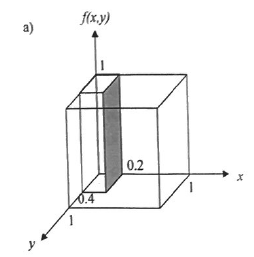
\includegraphics[width=0.5\linewidth,height=\textheight,keepaspectratio]{Material Quarto/Completa_files/Outras/Imagem4.png}

}

\caption{Função densidade de probabilidade conjunta
\label{figParticula}}

\end{figure}%

\subsection{Visualização gráfica: Var.
Contínuas}\label{visualizauxe7uxe3o-gruxe1fica-var.-contuxednuas}

Vejamos agora alguns gráficos de variáveis aleaórias bidimensionais:

\textbf{NORMAL BIVARIADA:}

Considere a variável aleatória \((X,Y)\) com distribuição normal
bivariada com a esperança de \(X\) igual a 10, de \(Y\) igual a 4, o
desvio-padrões iguais a 3 e 2 respectivamente. Aqui consideremaos a
correlação de 0.7 (veremos mais a frente esse conceito).

\begin{figure}[H]

{\centering 
\includegraphics[width=0.7\linewidth,height=\textheight,keepaspectratio]{cap6_va_bidimensional_files/figure-pdf/unnamed-chunk-4-1.pdf}

}

\caption{Distribuição conjunta normal bivariada}

\end{figure}%

\textbf{NORMAL BIVARIADA PADRÃO:}

Considere a variável aleatória \((X,Y)\) com distribuição normal
bivariada padrão, ou seja, a esperança de \(X\) e \(Y\) igual a a 1, o
desvio-padrões iguais a 1 e sem covariancia.

\begin{figure}[H]

{\centering 
\includegraphics[width=0.7\linewidth,height=\textheight,keepaspectratio]{cap6_va_bidimensional_files/figure-pdf/unnamed-chunk-5-1.pdf}

}

\caption{Distribuição conjunta normal padrão bivariada}

\end{figure}%

\section{Função Distribuição
Acumulada}\label{funuxe7uxe3o-distribuiuxe7uxe3o-acumulada}

Como no caso univariado a distinção entre variável aleatória conjunta
contínua e conjunta discreta pode ser feita em termos de sua função
distribuição conjunta acumulada.

\subsection{Caso discreto}\label{caso-discreto}

A função distribuição conjunta acumulada, F, da variável aleatória
bidimensional (X,Y) é definida por: \[\begin{array}{ccc}
 F(x,y)= P(X \leq x, Y \leq y) \ para \ -\infty < x_{i} < \infty \ e \ -\infty < y_{i} < \infty
\end{array}\]

Seja X e Y duas variáveis aleatórias discretas com função distribuição
conjunta \(F(x,y)\), a função distribuição conjunta acumulada de X e Y
será:

\[\begin{array}{ccc}
 F(x,y)=\sum_{f1=- \infty }^{x} \sum_{f2=- \infty }^{y}p(t_{1},t_{2})
\end{array}\]

Retomando os exemplos anteriores temos as seguintes funcÕes de
distribuição conjunta acumuladas discretas:

Para o caso dos dois dados apresentados anteriormente temos que:

\[F(2,3)=P(X\leq 2, Y \leq 3)=p(1,1)+p(1,2)+p(1,3)+p(2,1)+p(2,2)+p(2,3) \]

\[F(2,3)=P(X\leq 2, Y \leq 3)=6/36=1/6 \]

O gráfico segue abaixo.

\begin{figure}[H]

{\centering 
\includegraphics[width=0.7\linewidth,height=\textheight,keepaspectratio]{cap6_va_bidimensional_files/figure-pdf/unnamed-chunk-6-1.pdf}

}

\caption{Distribuição acumulada conjunta uniforme discreta}

\end{figure}%

Para o exemplo anterior (caixa do supermercado) encontre F(-1,2) e
F(1.5,2)

\begin{center}\rule{0.5\linewidth}{0.5pt}\end{center}

\[F(-1,2) = P(X \leq -1, Y \leq 2)= P(\emptyset)=0\]

*Note que é impossível no exemplo do caixa o valor assumir -1, portanto,
temos a probabilidade de um conjunto vazio, que será zero.

\begin{aligned}
F(1.5,2) &= P(X \leq 1.5, Y \leq 2) \\
         &= p(0,0)+p(0,1)+p(0,2)+p(1,0)+p(1,1)+p(1,2)=8/9
\end{aligned}

\subsection{Visualização gráfica}\label{visualizauxe7uxe3o-gruxe1fica-1}

\textbf{BINOMIAL:}

Considere a variável aleatória \((X,Y)\) com distribuição binomial e a
probabilidade de sucesso de \(X\) é igual a 0.75 e de \(Y\) igual a 0.25
com 10 rodadas, sua função distribuição acumulada será:

\begin{figure}[H]

{\centering 
\includegraphics[width=0.7\linewidth,height=\textheight,keepaspectratio]{cap6_va_bidimensional_files/figure-pdf/unnamed-chunk-7-1.pdf}

}

\caption{Distribuição conjunta Binomial}

\end{figure}%

\textbf{POISSON}\\
Considere a variável aleatória \((X,Y)\) com distribuição de poisson e o
valor esperado de \(X\) igual a 7, de \(Y\) igual a 4 e a covariância é
3 (a frente veremos esse conceito). Assim a função distribuição
acumulada será:

\begin{figure}[H]

{\centering 
\includegraphics[width=0.7\linewidth,height=\textheight,keepaspectratio]{cap6_va_bidimensional_files/figure-pdf/unnamed-chunk-8-1.pdf}

}

\caption{Distribuição conjunta de Poisson}

\end{figure}%

\subsection{Caso Contínuo}\label{caso-contuxednuo}

Seja X e Y duas variáveis aleatórias contínuas com função distribuição
conjunta \(F(x,y)\). Se existir uma função densidade de probabilidade
conjunta \(f(x,y)\) não negativa, assim a \textbf{função distribuição
conjunta acumulada de X e Y} será:

\[\begin{array}{ccc}
 F(x,y) = \int_{-\infty}^{x}\int_{- \infty}^{y} f(t_{1},t_{2})dt_{1}dt_{2} \ para \ -\infty < x_{i} < \infty \ e \ -\infty < y_{i} < \infty 
\end{array}\]

Para o exemplo anterior da partícula, encontre F(0.4, 0.4):

\begin{center}\rule{0.5\linewidth}{0.5pt}\end{center}

\textbf{Resposta:}

Ver figura abaixo. \[\begin{array}{ccc}
P(X \leq 0.4 ,Y \leq 0.4)= \int_{0}^{0.4}\int_{0}^{0.4}f(x,y)dxdy
\\
=\int_{0}^{0.4}\int_{0}^{0.4}1dxdy=\int_{0}^{0.4}(\int_{0}^{0.4}1dx)dy=\int_{0}^{0.4}(x\Big|_{0}^{0.4})dy
\\
=(0.4-0)\int_{0}^{0.4}dy=(0.4-0).(y\Big|_{0}^{0.4})\\
=(0.4-0)(0.4-0)=0.016
\\
P(X  \leq 0.4,Y \leq 0.4)=0.016
\end{array}\]

Seja \(X\) e \(Y\) duas variáveis aleatórias contínuas com função
distribuição conjunta \(F(x,y)\) então:

\[\begin{array}{ccc}
a) \ F(- \infty, - \infty )=  F(- \infty, y )=  F(x, - \infty )=0 \\
\end{array}\]

\[\begin{array}{ccc}
b) \ F(\infty, \infty ) = 1
\end{array}\]

No caso univariado tem-se: \[\begin{array}{ccc}
 f(x,y) = \frac{\partial^{2}F(x,y) }{\partial x \partial y} 
\end{array}\]

\subsection{Visualização gráfica}\label{visualizauxe7uxe3o-gruxe1fica-2}

Vejamos agora alguns gráficos de variáveis aleaórias bidimensionais:

\textbf{NORMAL BIVARIADA:}

Considere a variável aleatória \((X,Y)\) com distribuição normal
bivariada com a esperança de \(X\) igual a 10, de \(Y\) igual a 4, o
desvio-padrões iguais a 3 e 2 respectivamente. Aqui consideremaos a
correlação de 0.7 (veremos mais a frente esse conceito). Assim a função
distribuição acumulada conjunta terá o seguinte formato:

\begin{figure}[H]

{\centering 
\includegraphics[width=0.7\linewidth,height=\textheight,keepaspectratio]{cap6_va_bidimensional_files/figure-pdf/unnamed-chunk-9-1.pdf}

}

\caption{Distribuição acumulada conjunta normal}

\end{figure}%

\textbf{NORMAL BIVARIADA PADRÃO:} Considere a variável aleatória
\((X,Y)\) com distribuição normal bivariada padrão, ou seja, a esperança
de \(X\) e \(Y\) igual a a 1, o desvio-padrões iguais a 1 e sem
covariância. Assim a função distribuição acumulada conjunta terá o
seguinte formato:

\begin{figure}[H]

{\centering 
\includegraphics[width=0.7\linewidth,height=\textheight,keepaspectratio]{cap6_va_bidimensional_files/figure-pdf/unnamed-chunk-10-1.pdf}

}

\caption{Distribuição acumulada conjunta normal padrão}

\end{figure}%




\end{document}
